\section*{Team meeting report}

2018/07/20 - SYNALP - Esteban MARQUER

\subsection{Main points}

\begin{itemize}
\item
  Performance spike issue: see report
  ``2018\_07\_18-Performance\_spike\_analysis''

  \begin{itemize}
  \item
    solution chosen: replace hexadecimal codes with a special label per
    kind of code
  \end{itemize}
\item
  Long training: no over-fitting, 90\% accuracy in 500 epochs

  \begin{longtable}[]{@{}ll@{}}
  \hline
  sequence by sequence mesure & epoch summary\tabularnewline
  \hline
  \endhead
  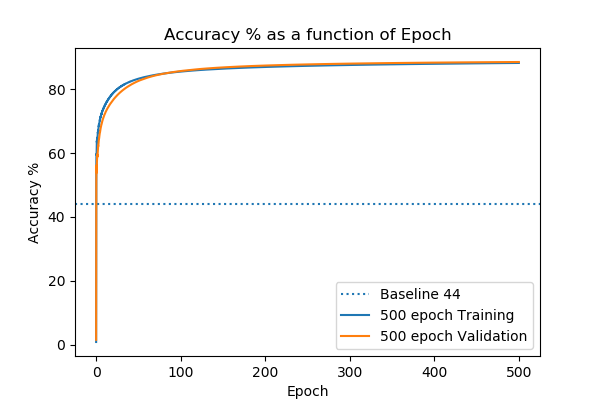
\includegraphics[width=.45\textwidth]{parts/appendix/reports-papud/2018_07_20-500_epochs/accuracy.png} &
  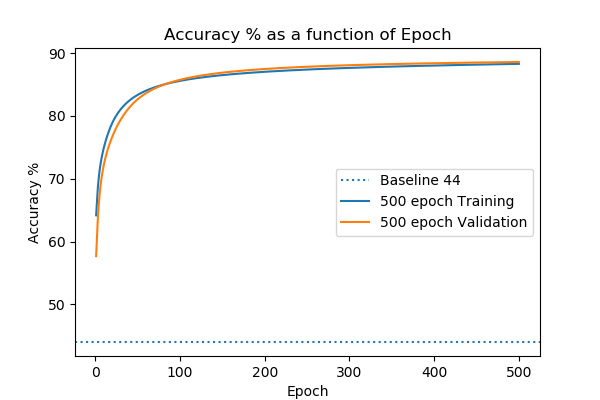
\includegraphics[width=.45\textwidth]{parts/appendix/reports-papud/2018_07_20-500_epochs/accuracy_epoch.png}\tabularnewline
  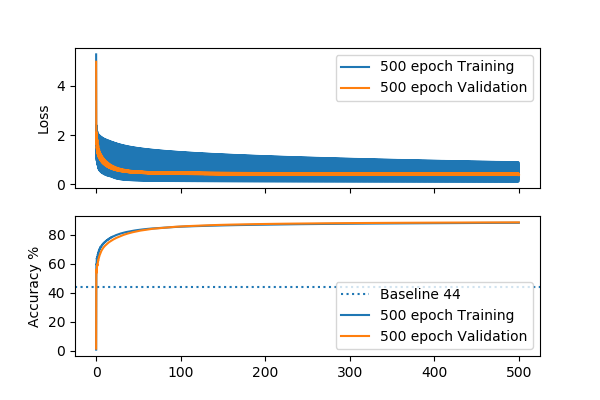
\includegraphics[width=.45\textwidth]{parts/appendix/reports-papud/2018_07_20-500_epochs/loss.png} &
  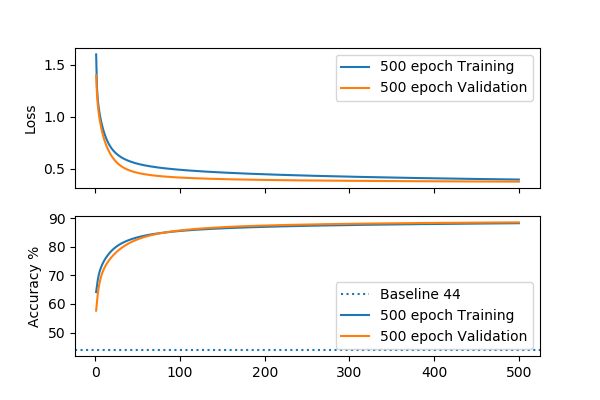
\includegraphics[width=.45\textwidth]{parts/appendix/reports-papud/2018_07_20-500_epochs/loss_epoch.png}\tabularnewline
  \hline
  \end{longtable}
\item
  Baseline accuracy: see first section of ``General\_information.md''
  for values.

  \begin{itemize}
  \item
    Baseline accuracy is high with padding (about 50\%), perhaps lines
    are too long (a lot of padding is needed)
  \item
    Compared with performance, performance is still good
  \end{itemize}
\item
  GPU usage with compleetely loaded corpus: 30\% to 60\%

  \begin{itemize}
  \item
    This is bad new, with such a model training should go at 99\% al the
    time
  \item
    It is necessary to locate the element slowing the process, try
    removing all unecessary processes (logging, storage in memory,
    accuracy, \ldots{})
  \end{itemize}
\item
  New corpus implementation (with buffer and iterators): about
  180s/epoch, 65s/epoch with old implementation (everything loaded in
  memory)

  \begin{itemize}
  \item
    a good implementation of the data loading is critical
  \item
    perhaps pre-loading is too slow because of computations, a
    pre-processed version could help
  \item
    training the model multiple time on a loaded segment could bridge
    the gap between the two processes used
  \item
    using more processes could do the trick (one for loading only, one
    for processing, and one for training)
  \item
    using ``binary''-sized batches (like 8, 64 or 1024) is said to
    achieve faster results, maybe a bit of speed can be gained there
  \end{itemize}
\item
  Development of a learning rate optimisation script: good, better if
  offline (good if both online and offline)

  \begin{itemize}
  \item
    online stands for optimisation before, or/and during every training
  \item
    offline stands for an analysis done a single time, aside from any
    training
  \end{itemize}
\end{itemize}

\subsection{Improvements and next
steps}

\begin{itemize}
\item
  Finish the development of learning rate optimisation.
\item
  Try to make the corpus implementation clean and fast enough (with
  compared run times).
\item
  Integrate the modifications of the corpus processing (memory address
  management)
\item
  Use ``binary''-sized batches; 128 seems perfect, as it is between 50
  and 200 (the bounds found when optimising batches).
\end{itemize}
